\documentclass{ctexart}
\usepackage{graphicx}
\usepackage{amsmath}
\usepackage{listings}
\usepackage[a4paper,left=3.18cm,right=3.18cm,top=2.54cm,bottom=2.54cm]{geometry}

\title{工科数学分析数学实验报告}
\author{Leo}
\date{\today}
% 18:07:45
%
%
%18:07:57
%ParametricPlot3D[{2*Cos[t], 2*Sin[t], 4*t}, {t, 0, 4*Pi}]
%
%18:08:08
%
%
%18:08:21
%NIntegrate[Exp[-x^2], {y, -1, 1}, {x, -1, 1}]
%
%18:08:29
%NIntegrate[Sin[x^2], {x, -2, 3}, {y, x^2, x + 6}]
%
%18:08:42
%t1 = ParametricPlot3D[{u, v, 0}, {u, -1, 1}, {v, -1, 2}, 
%AxesLabel -> {"X", "Y", "Z"}];
%
%t2 = ParametricPlot3D[{u^2, u, 0}, {u, -1, 1}, 
%AxesLabel -> {"X", "Y", "Z"}];
%
%t3 = ParametricPlot3D[{1, u, 0}, {u, -1, 1}, 
%AxesLabel -> {"X", "Y", "Z"}];
%
%Show[t1, t2, t3, PlotRange > {0, 1)]
%
%18:08:56
%Integrate[x y^2 z^2, {y, -1, 1}, {x, y^2, 1}, {z, 0, x^2 + y^2}]


\begin{document}
	\newcommand\dif{\mathrm{d}}
	\maketitle 
	\section{实验一}
	\subsection{实验题目}
	绘制螺旋线并观察图像特点。
	\subsection{实验目的及意义}
	利用数学软件Mathematica绘制三维图形来观察空间曲线图形的特点,提升空间想象能力。
	\subsection{程序设计}
	绘制空间曲线一般用参数式来表示。如果题目给出的是一般式
	\begin{equation}\label{key}
		\begin{cases}
			F(x,y,z)=0\\
			G(x,y,z)=0
		\end{cases}
	\end{equation}
则一般要先将$x,y$参数化,再代入上式将$z$参数化。本题中,设螺旋线参数方程为
\begin{equation}\label{key}
	\begin{cases}
		x=2\cos \theta\\
		y=2\sin \theta \\
		z= 4\theta
	\end{cases}
\end{equation}
式中$t \in [0,4\pi]$。其确定的空间曲线命令格式为
\begin{lstlisting}
	ParametricPlot3D[{x[t],y[t],z[t]},{t,tmin,tmax}]
\end{lstlisting}
在本题中为
\begin{lstlisting}
	ParametricPlot3D[{2*Cos[t],2*Sin[t],4*t},{t,0,4*Pi}]
\end{lstlisting}
\subsection{程序运行结果}
	如图是程序绘出的螺旋线图像。
\begin{figure}
	\centering
	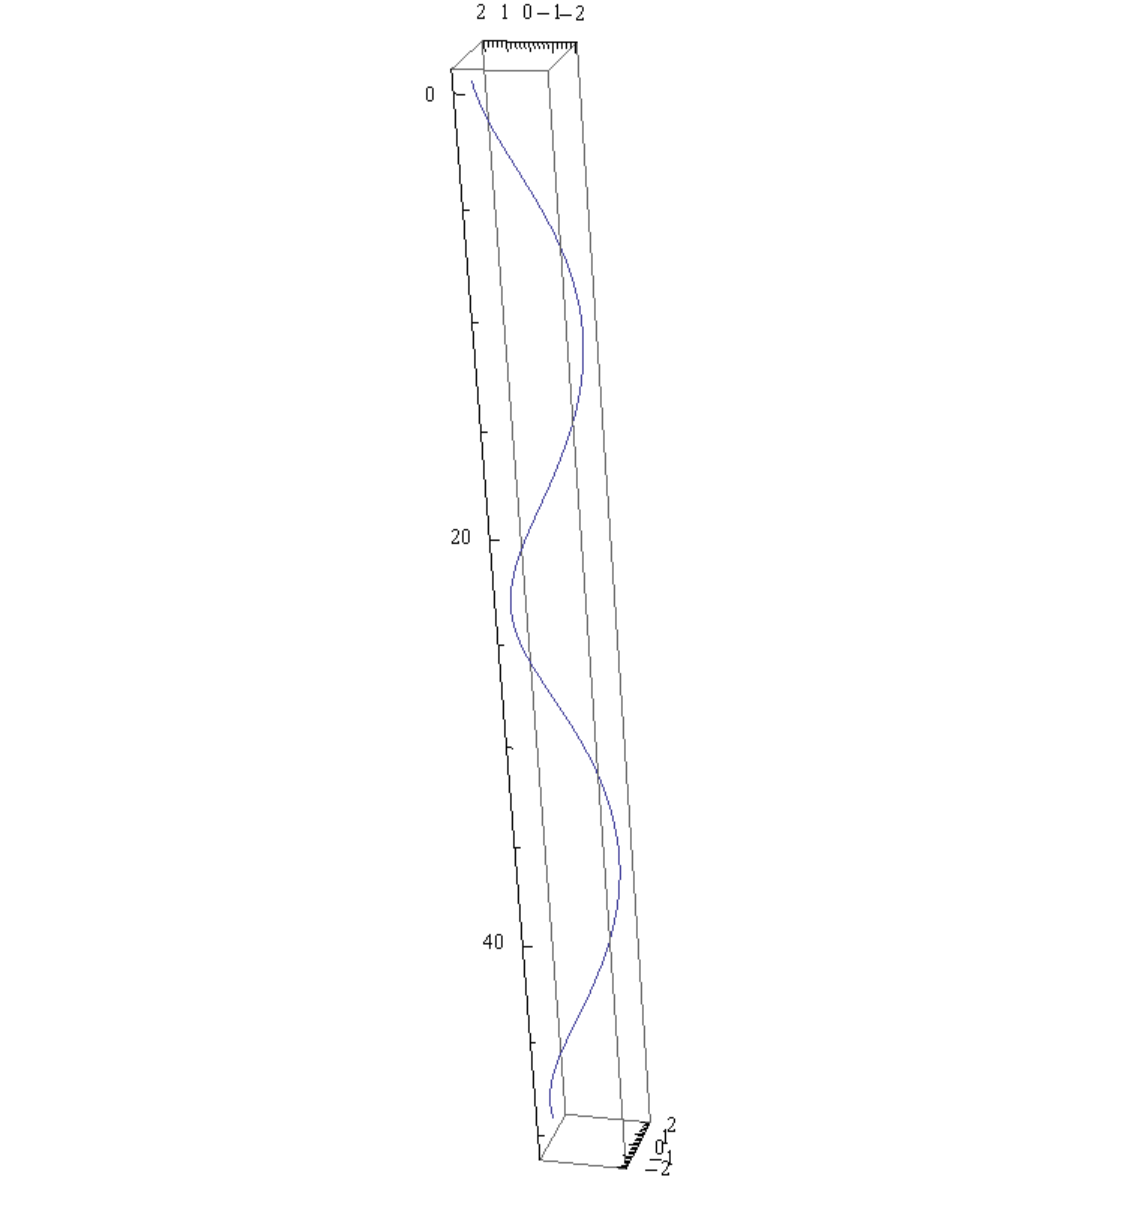
\includegraphics[scale=0.3]{E:/大学/课程/工科数学分析/数学实验报告/大一下/fig (2)}
	
	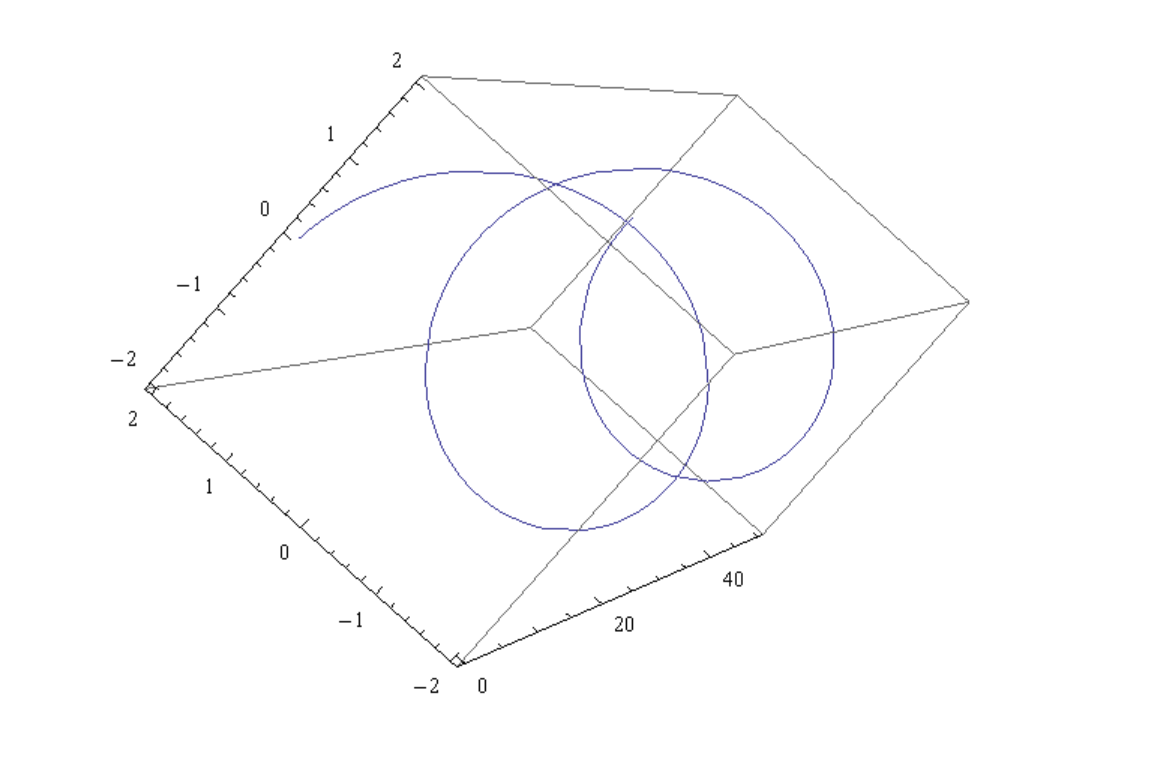
\includegraphics[scale=0.3]{E:/大学/课程/工科数学分析/数学实验报告/大一下/fig (4)}
\end{figure}
\newpage
	\subsection{结果分析与讨论}
	从图像的$z$轴方向看去,在$xOy$平面上呈圆形,半径为2;从侧面看图像螺旋上升,$z$方向上的速度恒定,总共转过两周。
	
	
	
	
\section{实验二}
\subsection{实验题目}
绘制上半球面并对空间曲面进行叠加和生成演示。
\subsection{实验目的及意义}
利用数学软件Mathematica绘制三维图形来观察空间曲面图形的特点,熟悉Mathematica的三维制图功能,为今后辅助学习打好基础。
\subsection{程序设计}
作一般式方程 $z = f (x, y)$ 所确定的曲面图形的 Mathematica 命令为:
\begin{lstlisting}
	Plot3D[f[x,y],{x,xmin,xmax},{y,ymin,ymax},options]
\end{lstlisting}
作参数方程
\begin{equation}\label{key}
	\begin{cases}
		x=x(u,v)\\
		y=y(u,v),\quad u\in [u_{min},u_{max}],v\in [v_{min},v_{max}] \\
		z=z(u,v)
	\end{cases}
\end{equation}
所确定的曲面图形的 Mathematica 命令为:
\begin{lstlisting}
	ParametricPlot3D[{x[u,v],y[u,v],z[u,v]},{u,umin,umax},
	{v,vmin,vmax},options]
\end{lstlisting}
首先我们选取绘图区间${-3<x<3,-4<y<4}$绘制上半球面$z=1+\sqrt{1-x^2-y^2}$的曲面。
\begin{lstlisting}
Plot3D[1 + Sqrt[1 - x^2 - y^2], {x, -1, 1}, {y, -1, 1}]
\end{lstlisting}
接下来我们将该球面和旋转抛物面$z=x^2+y^2$拼接。对应的参数方程为
\begin{equation}\label{key}
	\begin{cases}
		x=r \sin t\\
		y=r \cos t,t \in [0,2\pi],r\in [0,1]\\
		z=r^2
	\end{cases}
\end{equation}
\begin{equation}\label{key}
	\begin{cases}
		x=\cos u \sin v\\
		y=\sin u \sin v ,u\in [0,2\pi],v\in [0,2\pi]\\
		z=1+\cos v
	\end{cases}
\end{equation}
Mathematica中对应的命令为
\begin{lstlisting}
t1 = ParametricPlot3D[{r*Cos[t], r*Sin[t], r^2},
 {t, 0, 2*Pi}, {r, 0, 1}, PlotPoints -> 30];
t2 = ParametricPlot3D[{Cos[r]*Sin[t], Sin[r]*Sin[t]
	, 1 + Cos[t]}, {r, 0, 2*Pi}, {t, 0, Pi/2},
 PlotPoints -> 30];
tu = Show[t1, t2, PlotRange -> All]
\end{lstlisting}
最后用多页生成图像演示由曲线$y=\sin z,z \in [0,\pi]$绕$z$轴旋转产生旋转曲面的过程。先写出旋转面的方程:$x^2+y^2=\sin^2 z$,其参数形式为
\begin{equation}\label{key}
	\begin{cases}
		x=\sin z \cos u \\
		y=\sin z \sin u,z \in [0,\pi],u \in [0,2\pi]\\
		z=z
	\end{cases}
\end{equation}
Mathematica中对应的命令为
\begin{lstlisting}
	m=20;
	For[i=1,i<=m,i++,a=ParametricPlot3D[{Sin[z]*Cos[u]
		,Sin[z]*Sin[u],z},
	{z,0,Pi},{u,0,2Pi*i/m},AspectRatio->1,
	AxesLabel->{"X","Y","Z"},PlotPoint->30];Print[a]]
\end{lstlisting}
\subsection{程序运行结果}
如图分别给出从开始到结束的旋转面生成图像。\\
	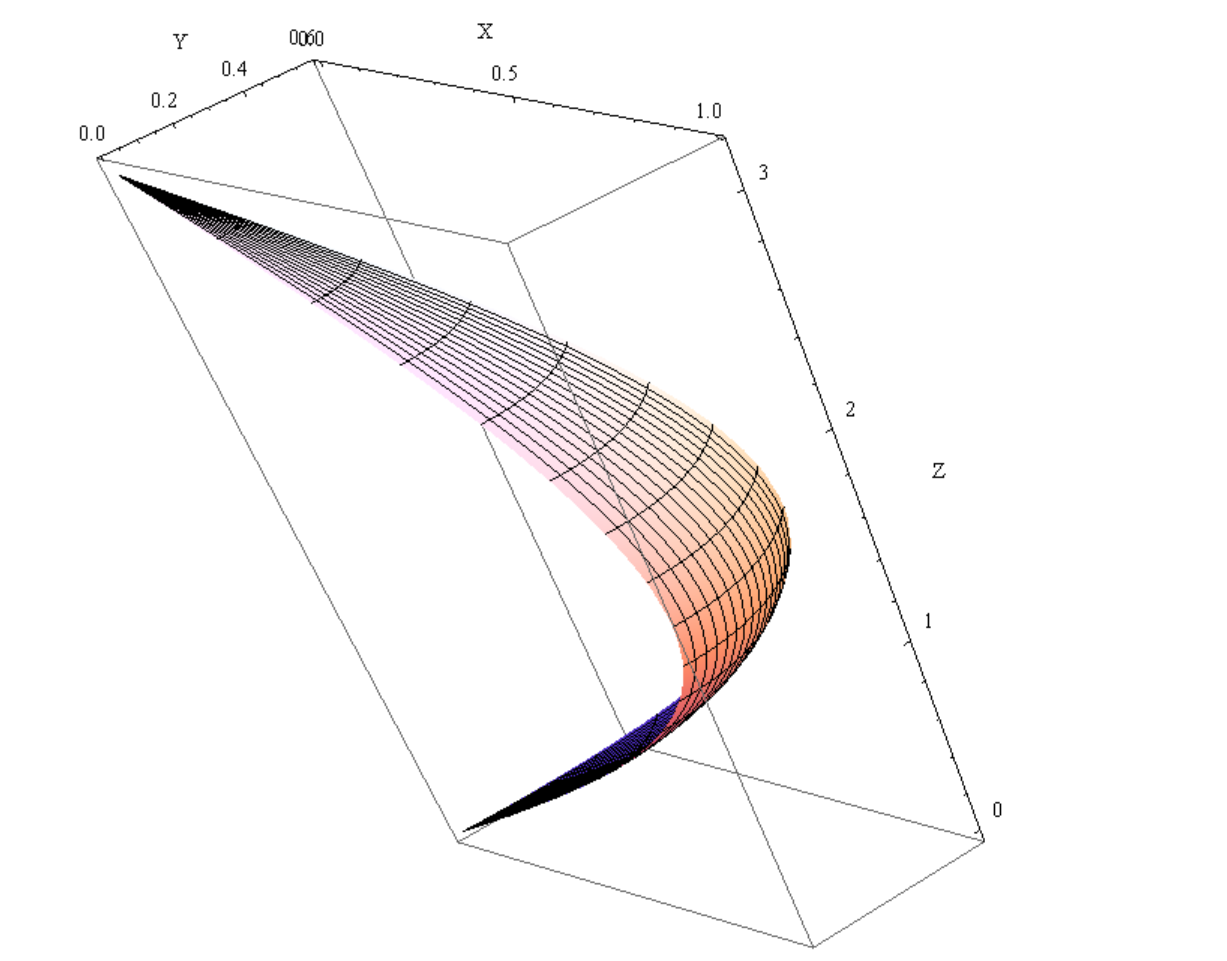
\includegraphics[scale=0.25]{E:/大学/课程/工科数学分析/数学实验报告/大一下/fig (6)}
	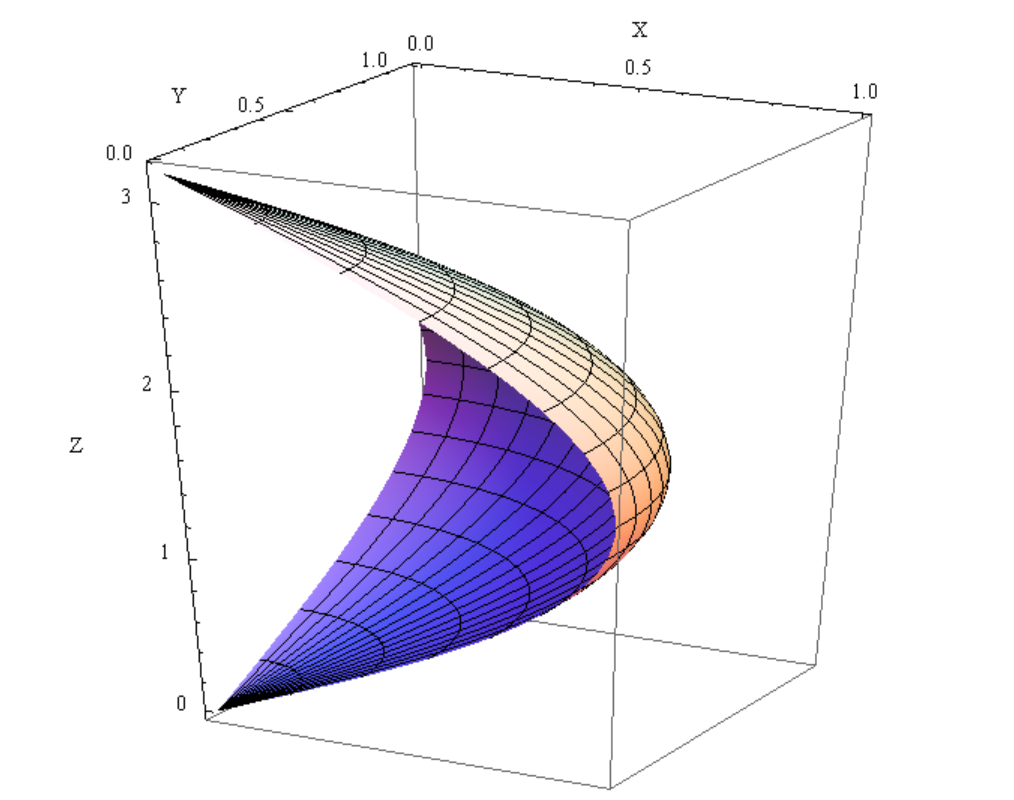
\includegraphics[scale=0.3]{E:/大学/课程/工科数学分析/数学实验报告/大一下/fig (3)}
	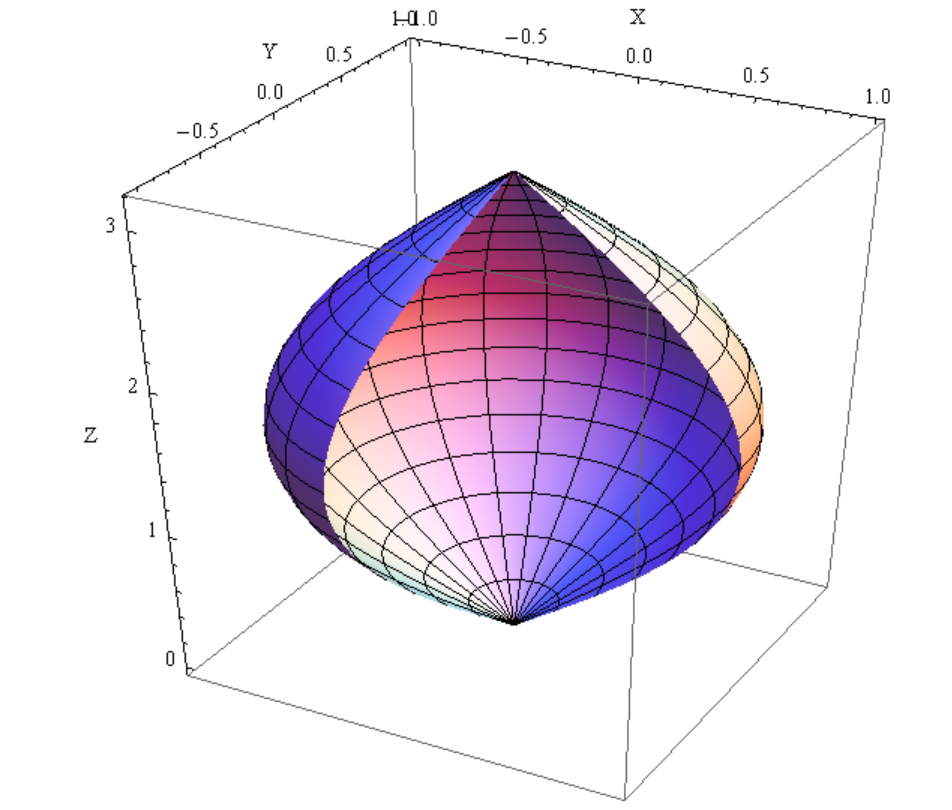
\includegraphics[scale=0.3]{E:/大学/课程/工科数学分析/数学实验报告/大一下/fig (8)}
	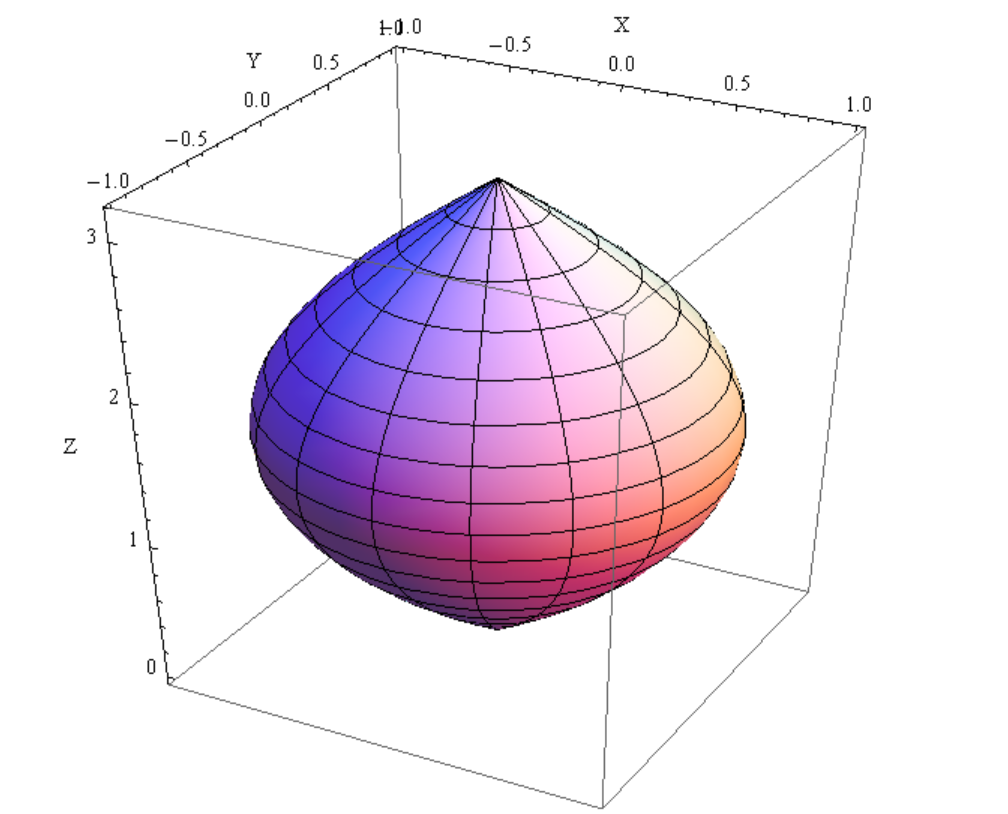
\includegraphics[scale=0.3]{E:/大学/课程/工科数学分析/数学实验报告/大一下/fig (5)}


\section{实验三}
\subsection{实验题目}
利用Mathematica进行重积分的数值计算。
\subsection{实验目的及意义}
借助形象化工具和计算工具,加深对重积分计算过程的理解,熟练掌握确定积分限的方法。
\subsection{程序设计}
\subsubsection{计算二重积分}
\noindent1.计算$\iint\limits_{D}e^{-x^2}\dif x \dif y$,积分域为矩形域$ |x|\leq 1,| y |\leq 1$。\\
2.计算$\iint\limits_{D}\sin x^2\dif x \dif y$,其中 D 是由直线 $y = x^2$ 和$ y = x + 6$ 围成的区域。\\
\textbf{解}\\
运行代码
\begin{lstlisting}
	NIntegrate[Exp[-x^2], {y, -1, 1}, {x, -1, 1}]
	NIntegrate[Sin[x^2], {x, -2, 3}, {y, x^2, x + 6}]
\end{lstlisting}
得到数值解2.9873与6.99628。

\subsubsection{计算三重积分}
\noindent3.求三重积分$\iiint \limits_{\Omega}xy^2z^2 \dif x\dif y \dif z$其中$\Omega$是由曲面 $z = x^2 + y^2,x = y^2,x = 1与 z = 0$所围成的立体区域。\\
\textbf{解}\\
为了便于确定积分域,我们先利用Mathematica绘图
\begin{lstlisting}
	s1 = ParametricPlot3D[{u, v, u^2 + v^2}, {u, -1, 1} ,
	
	{v, -1, 1}, PlotPoints - 50, AxesLabel , {}"X", "Y", "Z"} } ;
s2 = ParametricPlot3D[{u2, u, v}, {u, -1, 1}, {v, 0, 2},
	
	AxesLabel -> {"X", "Y", "Z"}] ;
	
	s3 = ParametricPlot3D[{1, u, v}, {u, -1, 1}, {v, 0, 2},
	
	AxesLabel-> {"X", "Y", "Z"}] ;
	
	s4 = ParametricPlot3D[{u, v, 0}, {u, -1, 1}, {v, -1, 1},
	
	AxesLabel-> {"X", "Y", "Z"}] ;
	
	Show[s1, s2, s3, s4]
\end{lstlisting}
运行后得到立体区域如图所示。\\
\begin{figure}[h]
	\centering
	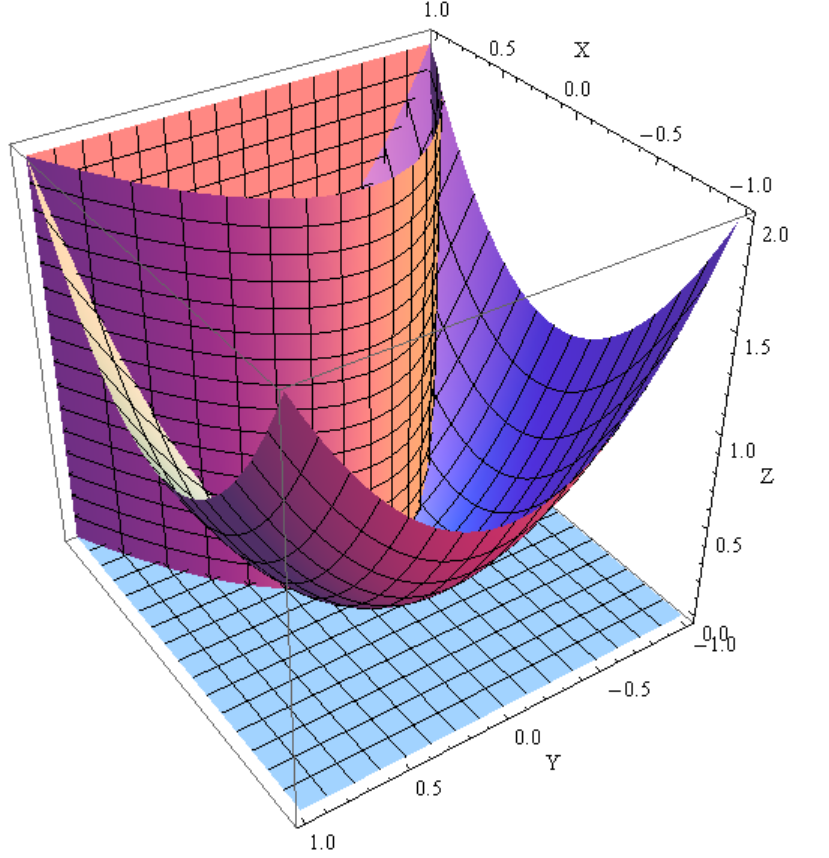
\includegraphics[scale=0.3]{E:/大学/课程/工科数学分析/数学实验报告/大一下/fig (9)}
\end{figure}

下面还要更清楚地看到积分域,则需要做投影图
\begin{lstlisting}
t1 = ParametricPlot3D[{u, v, 0}, {u, -1, 1}, {v, -1, 2}, 
AxesLabel -> {"X", "Y", "Z"}];

t2 = ParametricPlot3D[{u^2, u, 0}, {u, -1, 1}, 
AxesLabel -> {"X", "Y", "Z"}];

t3 = ParametricPlot3D[{1, u, 0}, {u, -1, 1}, 
AxesLabel -> {"X", "Y", "Z"}];

Show[t1, t2, t3, PlotRange > (0, 1)]
\end{lstlisting}
如图所示可以看出,$\Omega$ 在 $xOy$ 面的投影域为$ x = y^2,x = 1$所构成的平面区域\\
\begin{figure}
\centering
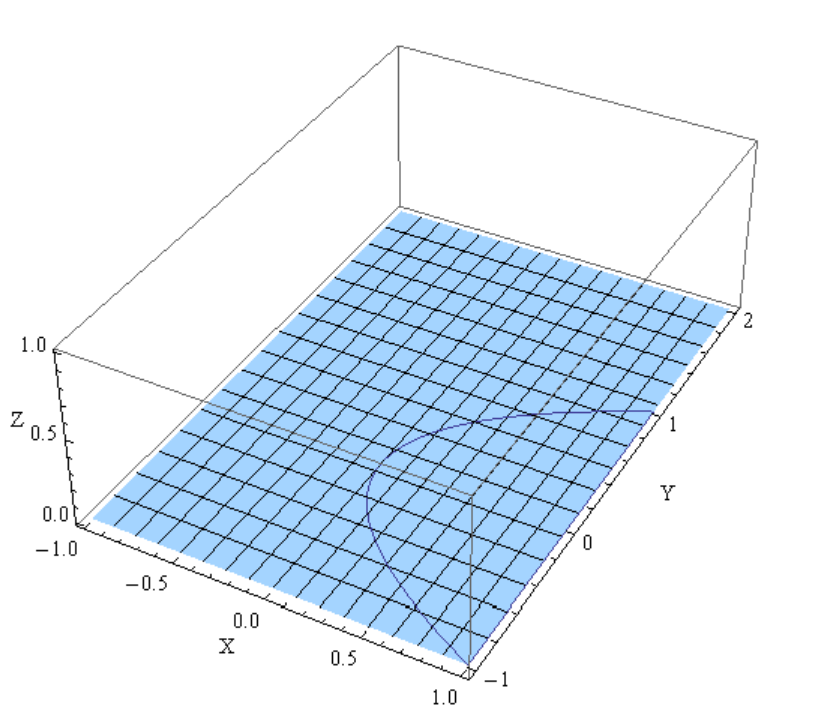
\includegraphics[scale=0.3]{E:/大学/课程/工科数学分析/数学实验报告/大一下/fig (10)}
\end{figure}\\
所以$\iiint \limits_{\Omega}xy^2z^2 \dif x\dif y \dif z=\int_{-1}^{1}\dif y\int_{y^2}^{1}\dif x\int_{0}^{x^2+y^2}xy^2z^2 \dif z$,利用代码实现
\begin{lstlisting}
Integrate[x y^2 z^2, {y, -1, 1}, {x, y^2, 1}, {z, 0, x^2 + y^2}]
\end{lstlisting}
得到所求三重积分的值为$\dfrac{475936}{3968055}$。
\end{document}